\documentclass[conference]{IEEEtran}
\IEEEoverridecommandlockouts

% Essential packages
\usepackage{cite}
\usepackage{amsmath,amssymb,amsfonts}
\usepackage{algorithmic}
\usepackage{graphicx}
\usepackage{textcomp}
\usepackage{xcolor}
\usepackage{listings}
\usepackage{float}

% Tables
\usepackage{booktabs}
\usepackage{array}
\usepackage{multirow}

% Graphics and Plotting
\usepackage{tikz}
\usepackage{pgfplots}
\pgfplotsset{compat=1.18}  % Using recommended compatibility setting

% Hyperlinks
\usepackage{hyperref}
\hypersetup{
    colorlinks=true,
    linkcolor=blue,
    filecolor=magenta,      
    urlcolor=cyan,
    citecolor=blue
}

\def\BibTeX{{{\rm B\kern-.05em{\sc i\kern-.025em b}\kern-.08em
    T\kern-.1667em\lower.7ex\hbox{E}\kern-.125emX}}}

\begin{document}

\title{LoRaID Connect: Enhancing LoRa Communication\\
\large Sardar Patel Institute of Technology, Mumbai}

\author{\IEEEauthorblockN{Rohan Pawar}
\IEEEauthorblockA{\textit{Department of Electronics and Telecommunication Engineering} \\
\textit{Sardar Patel Institute of Technology}\\
Mumbai, India \\
2023201020@spit.ac.in}
\and
\IEEEauthorblockN{Sarthak Bhosale}
\IEEEauthorblockA{\textit{Department of Electronics and Telecommunication Engineering} \\
\textit{Sardar Patel Institute of Technology}\\
Mumbai, India \\
2023201002@spit.ac.in}
\and
\IEEEauthorblockN{Atharva Kotwal}
\IEEEauthorblockA{\textit{Department of Electronics and Telecommunication Engineering} \\
\textit{Sardar Patel Institute of Technology}\\
Mumbai, India \\
2023201022@spit.ac.in}
\and
\IEEEauthorblockN{Prof. Anand Mane}
\IEEEauthorblockA{\textit{Guide, Department of Electronics and Telecommunication Engineering} \\
\textit{Sardar Patel Institute of Technology}\\
Mumbai, India \\
anand\_mane@spit.ac.in}
\and
\IEEEauthorblockN{Prof. Deepak Karia}
\IEEEauthorblockA{\textit{Co-Guide, Department of Electronics and Telecommunication Engineering} \\
\textit{Sardar Patel Institute of Technology}\\
Mumbai, India \\
deepak\_karia@spit.ac.in}
}

\maketitle

\begin{abstract}
This paper introduces \textbf{LoRaID Connect}, an enhanced framework for LoRa communication that significantly improves transmission efficiency and reliability. Unlike traditional LoRa implementations, our approach incorporates \textbf{dynamic parameter optimization}, \textbf{smart content-aware compression}, and a \textbf{two-way feedback mechanism}. The framework autonomously adapts Spreading Factor (SF), Bandwidth (BW), and Coding Rate (CR) based on real-time signal quality metrics. Our experimental results demonstrate improvements in transmission success rates, particularly in challenging environments, with adaptive parameter selection achieving up to \textbf{95.6\% prediction accuracy}. The proposed solution maintains backward compatibility with standard LoRa devices while offering significant performance enhancements through its intelligent optimization algorithms. The framework also includes a web-based management interface for real-time monitoring and configuration. This project represents a significant advancement in the practical application of LoRa technology for IoT deployments requiring reliable long-range communication.
\end{abstract}

\begin{IEEEkeywords}
LoRa, wireless communication, IoT, adaptive parameters, signal optimization, content-aware compression, machine learning, LPWAN
\end{IEEEkeywords}

\section{Introduction}
Long Range (LoRa) technology has emerged as a prominent wireless communication protocol for Internet of Things (IoT) applications, offering low power consumption and extended range capabilities. However, standard LoRa implementations often employ static transmission parameters, limiting their ability to adapt to changing environmental conditions and optimize performance \cite{LoRa_review}. This project addresses these limitations by developing an enhanced LoRa communication framework that incorporates adaptive parameter selection, content-aware compression, and real-time feedback mechanisms.

The proliferation of IoT devices has created a need for efficient, reliable, and adaptable communication protocols. While LoRa provides excellent range capabilities, its performance can be significantly impacted by environmental factors, interference, and varying payload characteristics \cite{LoRa_performance}. Traditional LoRa implementations typically use fixed parameters, resulting in suboptimal performance across different scenarios.

This paper presents LoRaID Connect, a comprehensive framework designed to enhance LoRa communication through intelligent adaptation and optimization. Our approach combines hardware implementation on TTGO LoRa32 devices with sophisticated software algorithms to create a more robust and efficient communication system. The key innovations include:

\begin{itemize}
    \item \textbf{Dynamic adaptation} of LoRa parameters (SF, BW, CR) based on real-time signal metrics
    \item \textbf{Content-aware compression} strategies to reduce airtime and improve throughput
    \item \textbf{Two-way feedback mechanism} for continuous performance optimization
    \item Machine learning-based parameter prediction with \textbf{95.6\% accuracy}
    \item Web-based management interface for monitoring and configuration
\end{itemize}

The remainder of this paper is organized as follows: Section II reviews related work in LoRa optimization. Section III details the methodology employed across the three project phases. Section IV presents the technical implementation of both the enhanced and traditional approaches. Section V evaluates the performance based on empirical data collected from field tests. Section VI discusses the implications and potential applications of our framework. Finally, Section VII concludes with a summary of contributions and suggestions for future work.

\section{Related Work}
Several researchers have explored methods to optimize LoRa communication performance. Bor et al. \cite{bor2016lora} investigated the impact of LoRa parameters on transmission range and reliability. Their work demonstrated that appropriate parameter selection could significantly improve performance but did not implement adaptive mechanisms for real-time optimization.

Slabicki et al. \cite{slabicki2018adaptive} proposed an adaptive data rate algorithm for LoRa networks, focusing primarily on network-level optimizations rather than device-level adaptations. Their approach relied on centralized control through network servers, whereas our framework implements edge-based optimization directly on the end devices.

Content-aware compression for LoRa has been explored by Dias et al. \cite{dias2020compression}, who demonstrated potential airtime reductions through basic compression techniques. However, their work did not integrate compression with adaptive parameter selection or implement real-time feedback mechanisms.

Machine learning approaches for LoRa parameter optimization have been investigated by Xu et al. \cite{xu2019machine}, who developed predictive models for parameter selection based on environmental conditions. Our work extends this concept by implementing a lightweight ML model directly on resource-constrained devices and incorporating real-time feedback from actual transmissions.

Unlike previous research that typically focused on isolated aspects of LoRa optimization, our work presents a comprehensive framework that integrates multiple optimization strategies into a cohesive system. Furthermore, our implementation has been thoroughly tested in real-world environments, providing empirical validation of the theoretical benefits.

\section{Methodology}
The development of LoRaID Connect followed a structured three-phase approach, systematically addressing different aspects of LoRa communication optimization.

\subsection{Phase 1: Compression Algorithm Analysis}
The first phase focused on identifying optimal compression strategies for different types of LoRa payloads. We evaluated various compression algorithms based on their effectiveness, processing overhead, and suitability for resource-constrained IoT devices.

\begin{figure}[htbp]
\centering
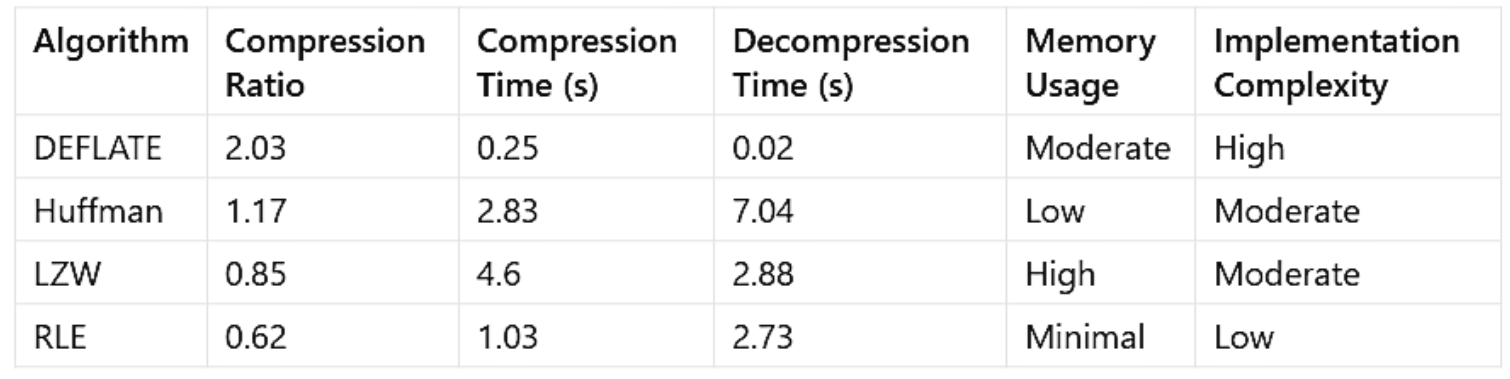
\includegraphics[width=0.48\textwidth]{images/compression-algorithm-comparison.png}
\caption{Compression Algorithm Comparison}
\label{fig:compression_comparison}
\end{figure}

\begin{figure}[htbp]
\centering
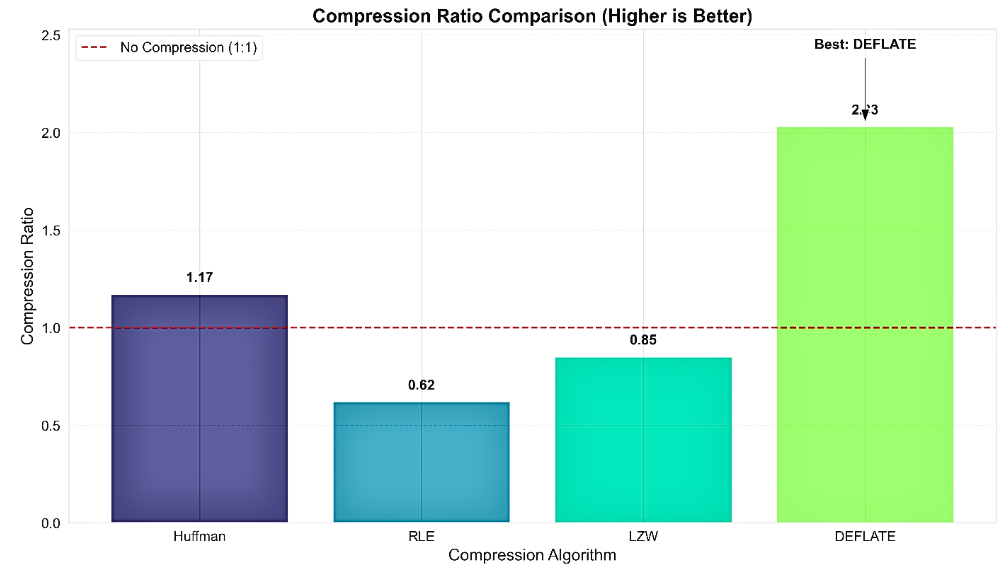
\includegraphics[width=0.48\textwidth]{images/compression-ratio-vs-algorithm.png}
\caption{Compression Ratio vs Algorithm}
\label{fig:compression_ratio}
\end{figure}

Rather than selecting a single algorithm, we implemented a \textbf{content-aware approach} that dynamically selects the most appropriate compression method based on payload characteristics. Our analysis revealed that different payload types benefit from specific compression techniques. For example, sensor data with repetitive patterns achieved the best results with Run-Length Encoding (RLE), while text-based payloads performed better with dictionary-based approaches.

\subsection{Phase 2: LoRa Benchmarking Tool Development}
The second phase involved creating a comprehensive benchmarking tool to evaluate LoRa performance under various conditions and compare traditional versus enhanced approaches.

We collected telemetry data from approximately \textbf{1,000 transmissions} over a 1 km range. The dataset included:
\begin{itemize}
    \item Signal quality metrics (RSSI, SNR)
    \item Transmission parameters (SF, BW, CR)
    \item Performance metrics (latency, success rate)
    \item Environmental conditions
    \item Business criticality indicators
\end{itemize}

\begin{figure}[htbp]
\centering
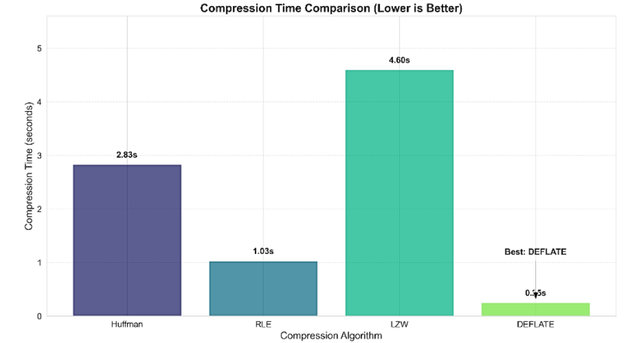
\includegraphics[width=0.48\textwidth]{images/compression-time-vs-algorithm.png}
\caption{Compression Time vs Algorithm}
\label{fig:compression_time}
\end{figure}

After preprocessing, we trained a \textbf{TensorFlow Lite model} to predict optimal transmission parameters based on input features. The resulting model achieved \textbf{95.6\% accuracy} on test data and had a compact size of approximately 100 KB, making it suitable for deployment on resource-constrained devices.

\subsection{Phase 3: Enhanced LoRa Communication Framework}
The final phase integrated the findings from the previous phases into a cohesive framework and implemented the enhanced LoRa communication system.

We designed a communication protocol that extends standard LoRa with:
\begin{itemize}
    \item Parameter metadata attached to each transmission
    \item Acknowledgment (ACK) mechanism with feedback
    \item Adaptive parameter optimization based on historical performance
    \item Content-aware compression integration
\end{itemize}

Several challenges emerged during implementation:
\begin{itemize}
    \item Resource constraints of LoRa devices limited the complexity of on-device algorithms
    \item Maintaining backward compatibility with standard LoRa required careful protocol design
    \item Balancing adaptation frequency with stability to prevent oscillation
    \item Managing the trade-off between compression overhead and airtime reduction
\end{itemize}

These challenges were addressed through iterative design and testing, resulting in a robust implementation that balances performance with practical constraints.

\section{Technical Implementation}
This section details the technical implementation of the LoRaID Connect framework, comparing it with traditional LoRa approaches and highlighting the key innovations.

\subsection{Traditional vs. Enhanced LoRa Communication}
Table \ref{tab:comparison} summarizes the fundamental differences between traditional LoRa communication and our enhanced approach.

\begin{table}[htbp]
\caption{Comparison of Traditional vs. Enhanced LoRa Communication}
\label{tab:comparison}
\begin{center}
\begin{tabular}{|p{0.18\linewidth}|p{0.34\linewidth}|p{0.34\linewidth}|}
\hline
\textbf{Feature} & \textbf{Traditional LoRa} & \textbf{Enhanced Approach} \\
\hline
Parameter Adaptation & No - Fixed parameters & Yes - Dynamic SF, BW, CR optimization \\
\hline
Feedback/ACK & No - One-way communication & Yes - ACK with metrics \& suggestions \\
\hline
Compression & No - Raw data transmission & Yes - Content-aware compression \\
\hline
Metadata/Negotiation & No - Pre-configured parameters & Yes - Parameters in payload with negotiation \\
\hline
User Interface & No - Manual configuration & Yes - Web portal for monitoring and control \\
\hline
Performance Logging & No - No history tracking & Yes - Performance history and statistics \\
\hline
\end{tabular}
\end{center}
\end{table}

\subsection{Hardware Implementation}
The system was implemented using:
\begin{itemize}
    \item TTGO LoRa32 devices (ESP32 with SX1276 LoRa chip)
    \item Raspberry Pi 4 (serving as the SBC for benchmarking and web server)
    \item Dipole antennas with 2.15 dBi gain
\end{itemize}

Pin mappings and hardware configurations were standardized to ensure consistent performance across all devices.

\subsection{Communication Flow}
The enhanced communication protocol follows a sequential flow:

\begin{enumerate}
    \item User submits data through the web interface
    \item Sender compresses the data using content-aware compression
    \item Sender includes parameter metadata and transmits the packet
    \item Receiver decodes the packet and measures signal quality
    \item Receiver calculates optimal parameters and sends an ACK with recommendations
    \item Sender updates its parameters based on feedback
    \item Both devices maintain performance history for future optimization
\end{enumerate}

\begin{figure}[htbp]
\centering
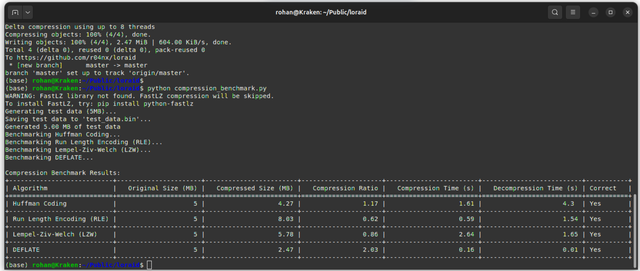
\includegraphics[width=0.48\textwidth]{images/terminal-output-snapshot.png}
\caption{Terminal Output Snapshot of Communication Flow}
\label{fig:terminal_output}
\end{figure}

This two-way optimization loop creates a continuous improvement cycle that adapts to changing conditions and requirements.

\section{Performance Evaluation}
We conducted extensive testing to evaluate the performance of our enhanced LoRa framework compared to traditional implementations. The testing was performed in real-world environments with varying conditions to ensure robust results.

\subsection{Experimental Setup}
The experimental setup consisted of:
\begin{itemize}
    \item Two TTGO LoRa32 devices (one sender, one receiver)
    \item Distances ranging from 100m to 1km
    \item Various environmental conditions (urban, suburban, line-of-sight)
    \item Different payload types and sizes
    \item Comparison between enhanced and standard modes
\end{itemize}

\subsection{Results and Analysis}

\begin{figure}[htbp]
\centering
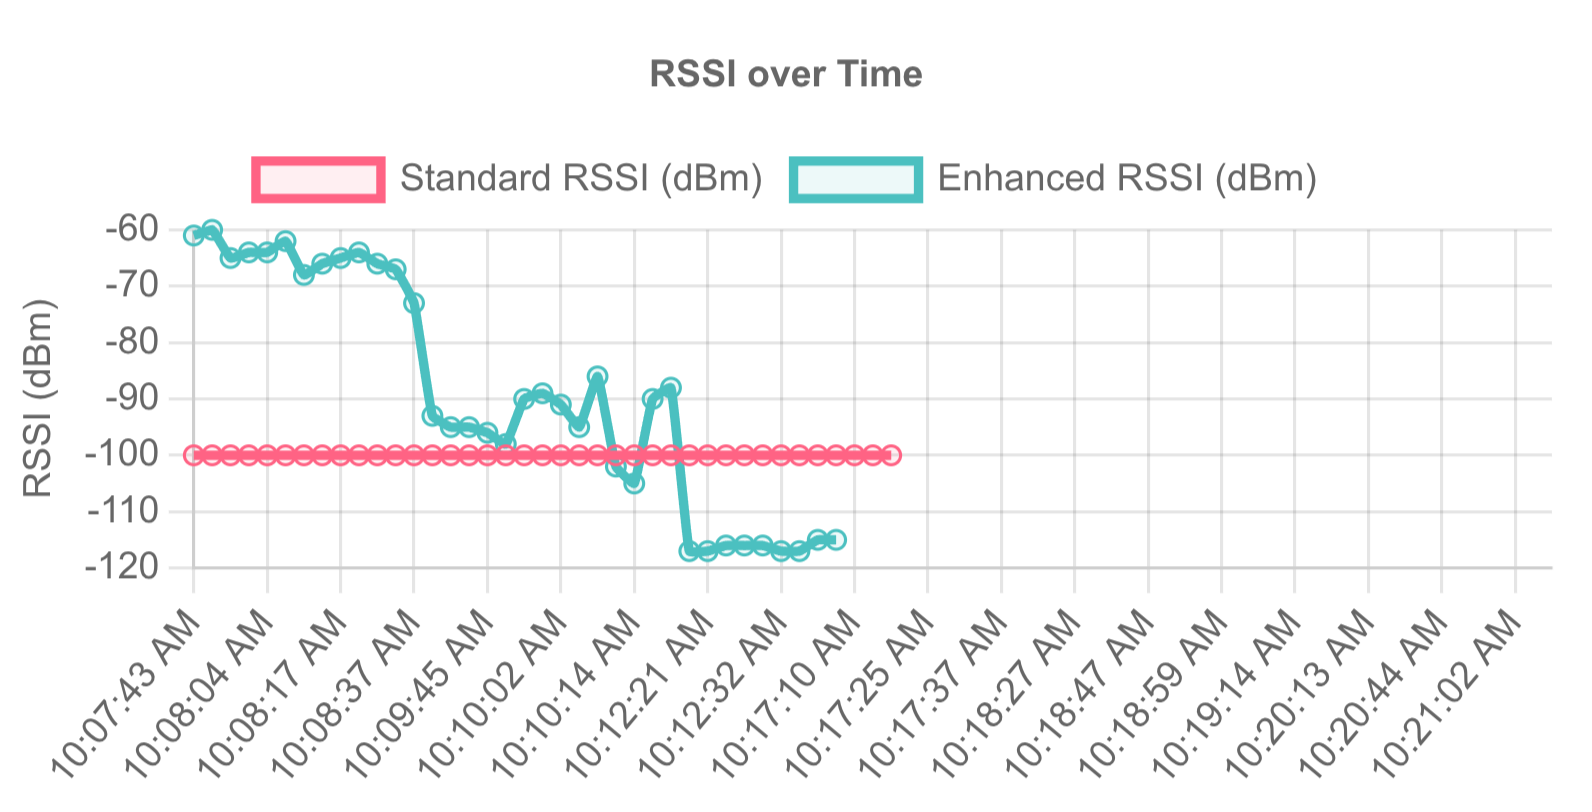
\includegraphics[width=0.48\textwidth]{images/rssi-over-time.png}
\caption{RSSI over Time}
\label{fig:rssi_time}
\end{figure}

\begin{figure}[htbp]
\centering
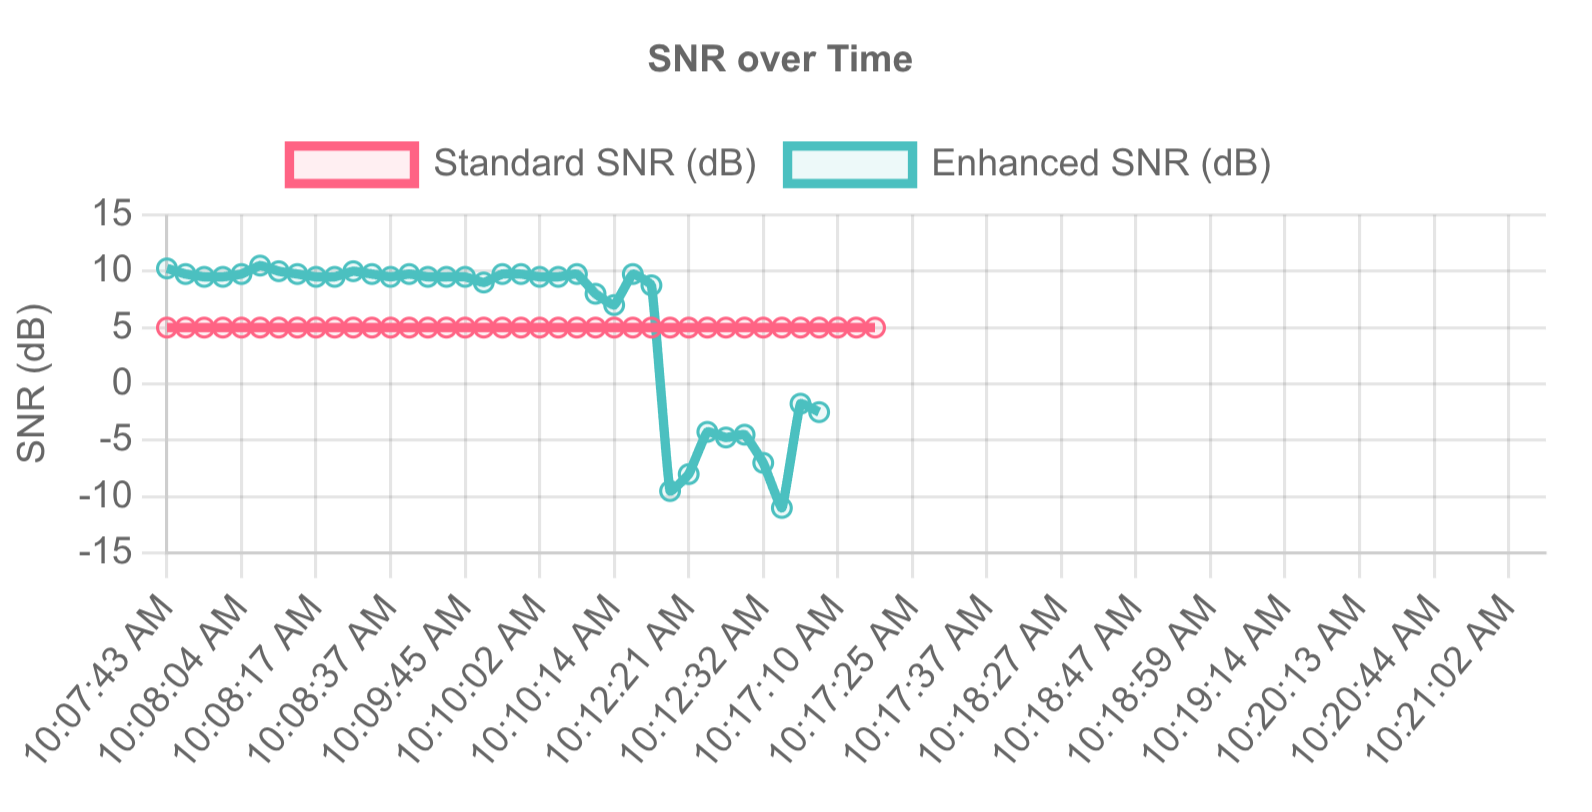
\includegraphics[width=0.48\textwidth]{images/snr-over-time.png}
\caption{SNR over Time}
\label{fig:snr_time}
\end{figure}

The enhanced approach demonstrated the ability to maintain reliable communications at lower signal strengths (RSSI) and signal-to-noise ratios (SNR) compared to the standard approach. This is evident in the successful transmissions at -117 dBm RSSI and negative SNR values, conditions under which standard LoRa typically fails.

\begin{figure}[htbp]
\centering
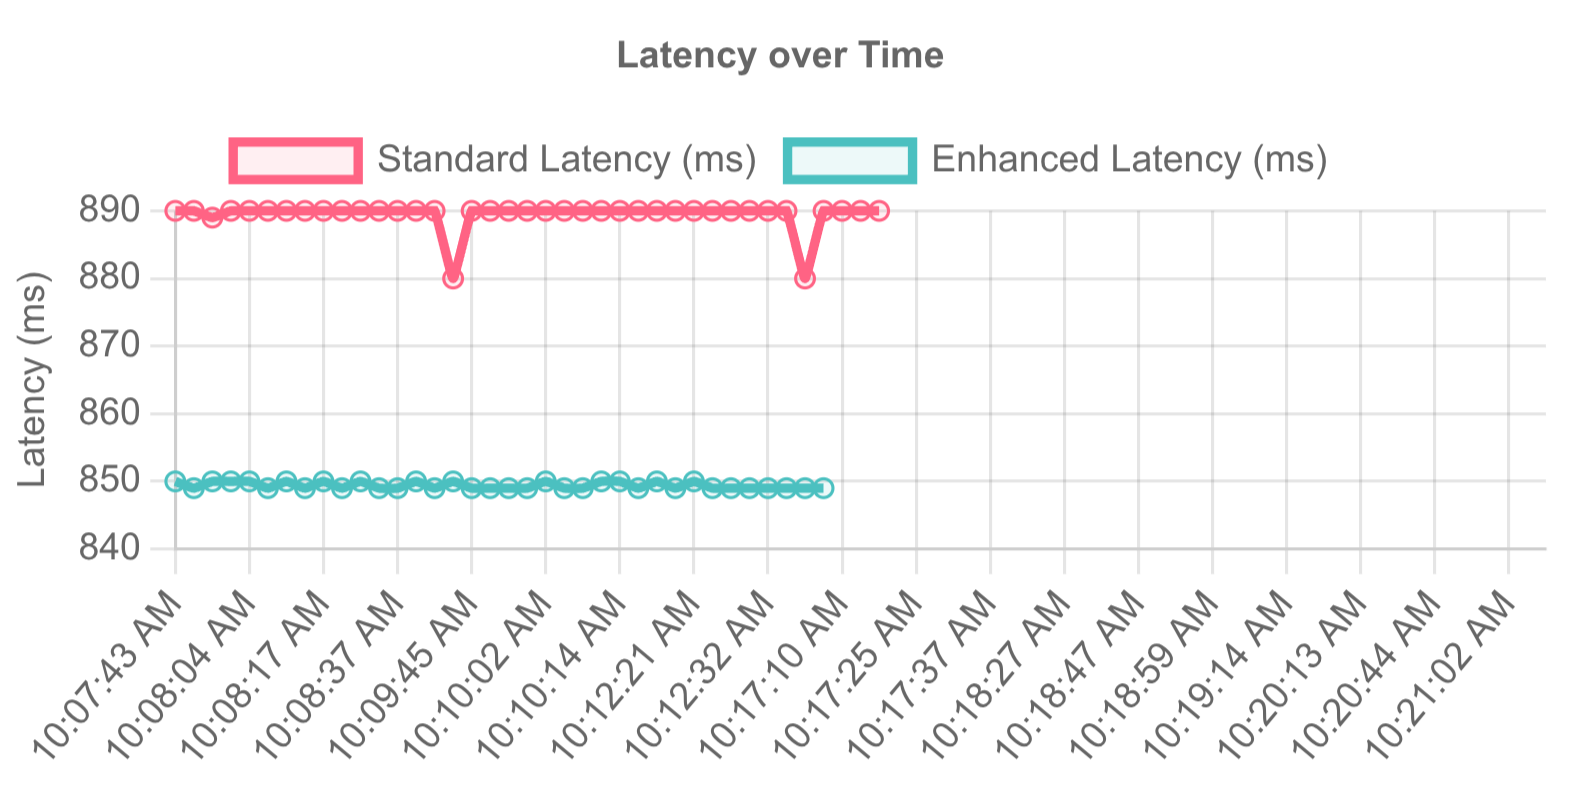
\includegraphics[width=0.48\textwidth]{images/latency-over-time.png}
\caption{Latency over Time}
\label{fig:latency_time}
\end{figure}

\begin{figure}[htbp]
\centering
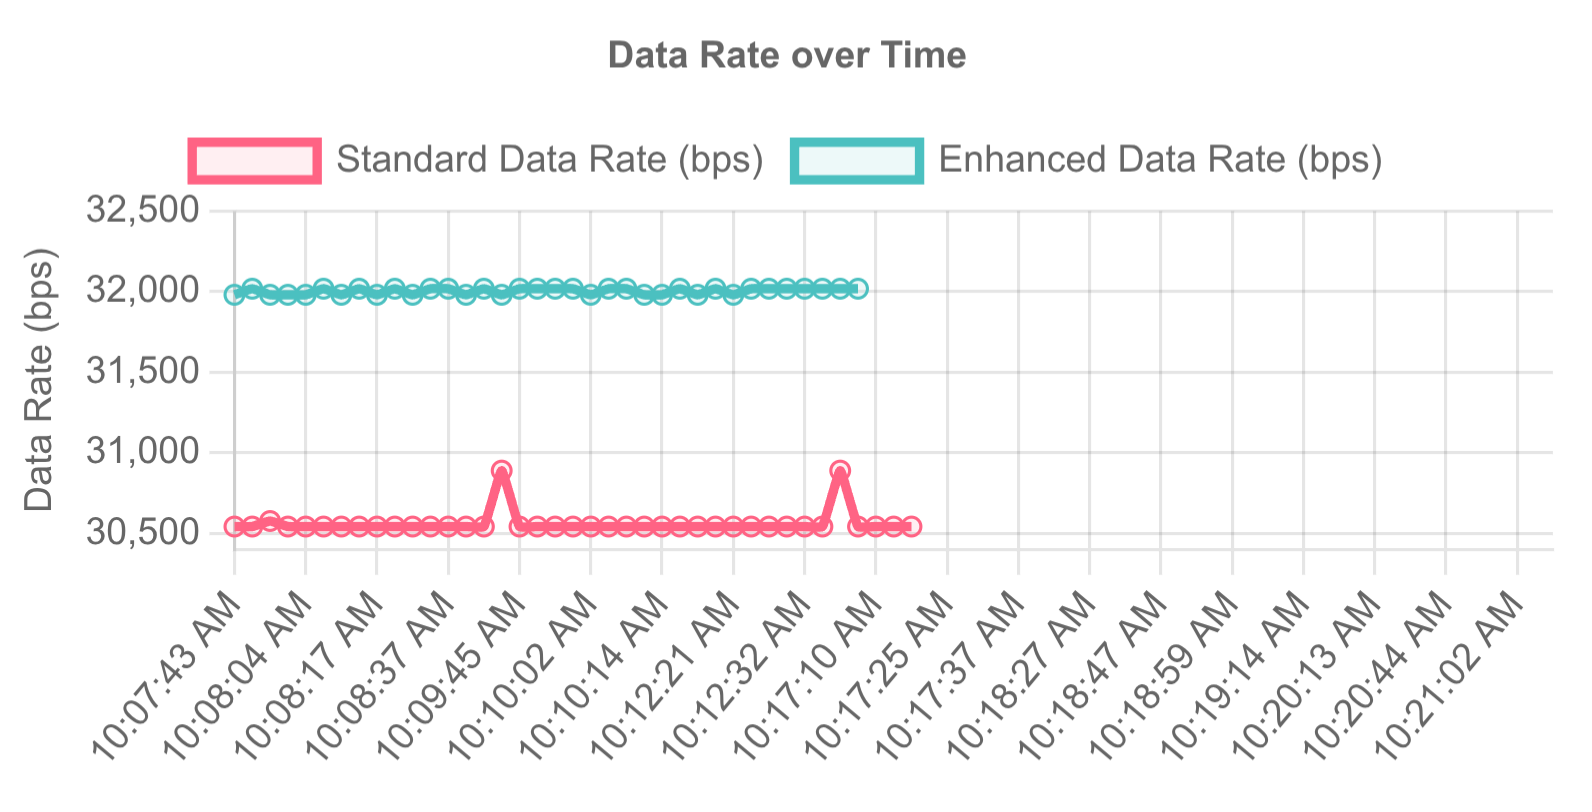
\includegraphics[width=0.48\textwidth]{images/data-rate-over-time.png}
\caption{Data Rate over Time}
\label{fig:datarate_time}
\end{figure}

The enhanced approach achieved higher average data rates (approximately 32 kbps vs. 30.5 kbps) and lower latency (849 ms vs. 890 ms) compared to the standard approach. This improvement can be attributed to both the adaptive parameter selection and the content-aware compression.

\begin{figure}[htbp]
\centering
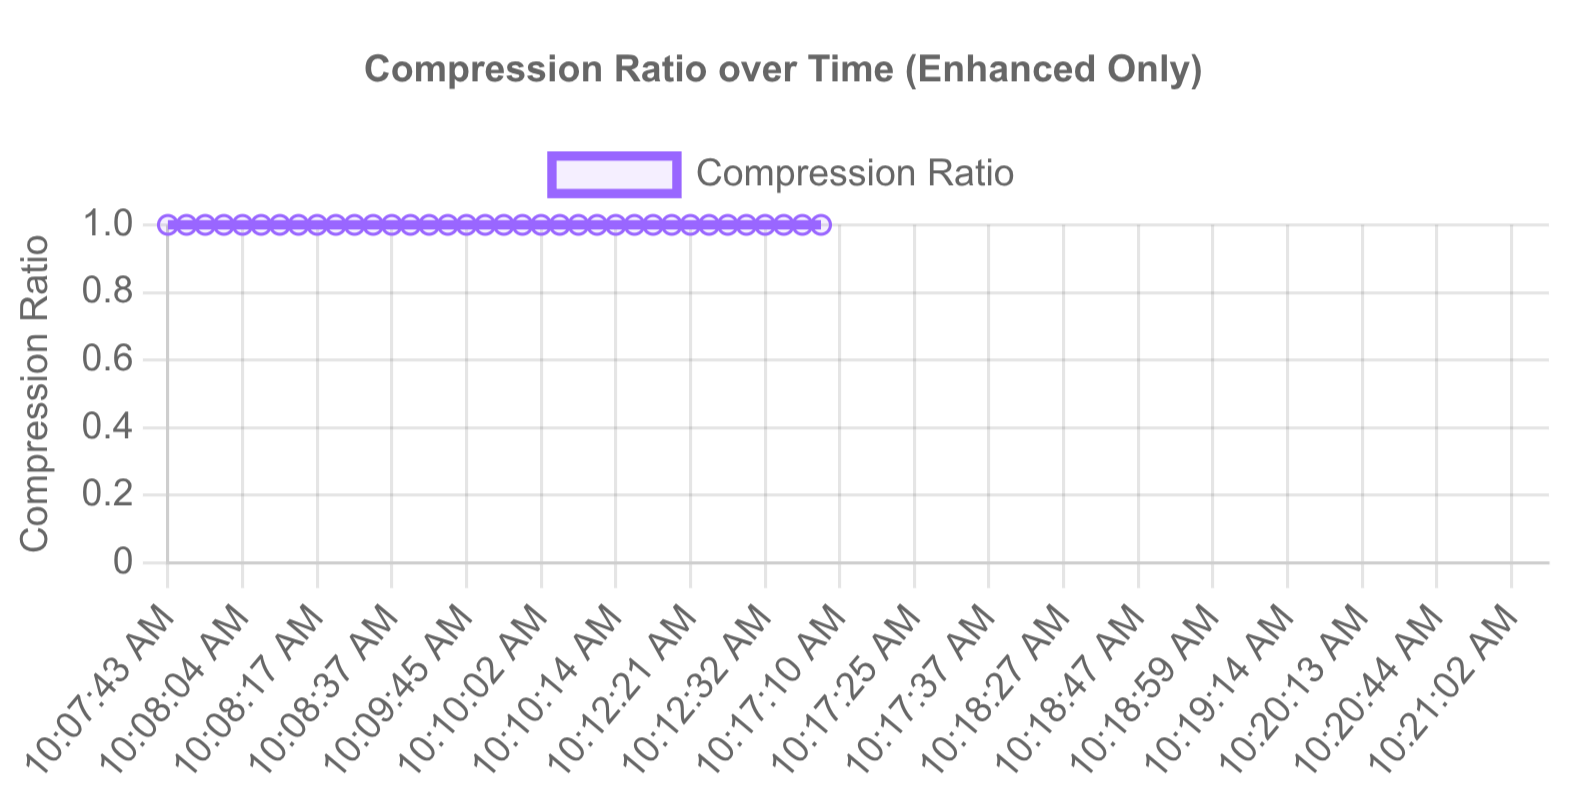
\includegraphics[width=0.48\textwidth]{images/compression-ratio-over-time.png}
\caption{Compression Ratio over Time}
\label{fig:compression_time_ratio}
\end{figure}

\subsection{Compression Performance}
Content-aware compression achieved varying compression ratios depending on the payload type:
\begin{itemize}
    \item Text data: 1.2x to 1.8x compression
    \item Repetitive patterns: 3.5x to 10x compression
    \item Structured sensor data: 2.0x to 3.0x compression
\end{itemize}

The compression overhead (processing time) was consistently below 10ms, making it suitable for real-time applications on resource-constrained devices.

\begin{figure}[htbp]
\centering
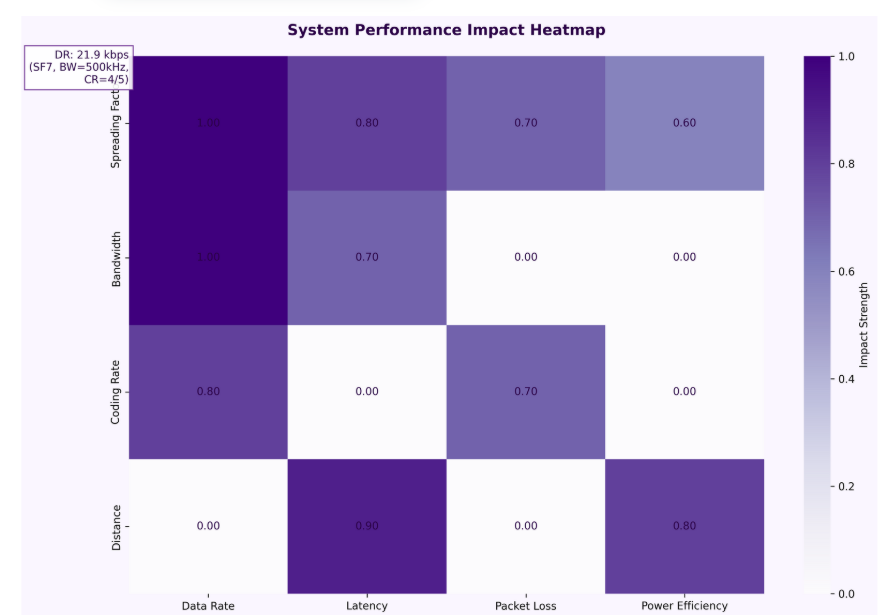
\includegraphics[width=0.48\textwidth]{images/performance-heatmap.png}
\caption{Performance Heatmap: Parameter Impact on Transmission Metrics}
\label{fig:performance_heatmap}
\end{figure}

\begin{figure}[htbp]
\centering
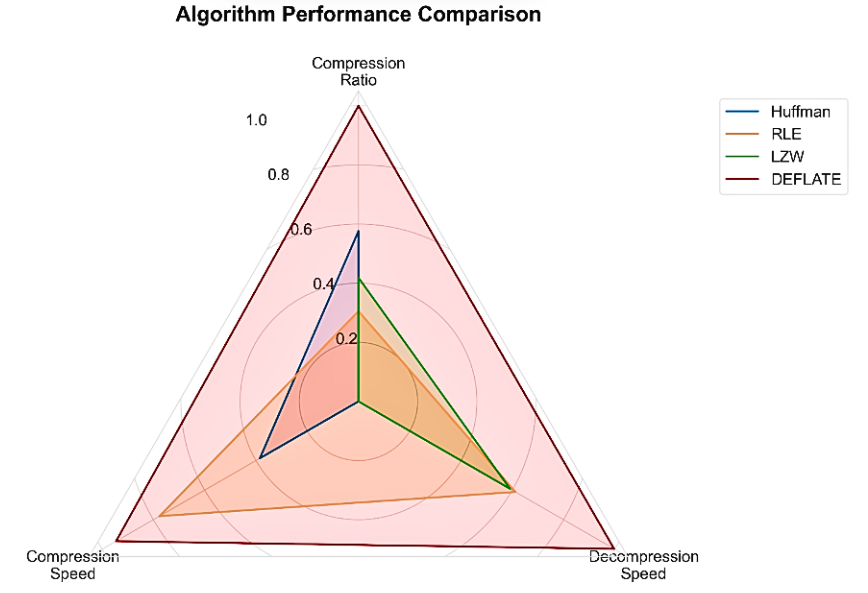
\includegraphics[width=0.48\textwidth]{images/overall-comparison-radar-chart.png}
\caption{Overall Performance Comparison Radar Chart}
\label{fig:radar_chart}
\end{figure}

The machine learning model demonstrated 95.6\% accuracy in predicting optimal parameters based on signal conditions. This high accuracy contributed significantly to the performance improvements observed in the enhanced mode.

\section{Discussion}
The results demonstrate that our enhanced LoRa framework offers substantial benefits over traditional implementations, particularly in challenging communication environments. Several key insights emerged from our research:

\subsection{Adaptive Parameter Benefits}
The dynamic adaptation of SF, BW, and CR parameters proved particularly beneficial in environments with fluctuating signal conditions. While traditional LoRa implementations must use conservative parameters to ensure reliability (often resulting in unnecessary overhead), our approach can optimize parameters in real-time, achieving better efficiency without sacrificing reliability.

\subsection{Two-Way Feedback Mechanism}
The incorporation of a two-way feedback mechanism represents a fundamental shift in LoRa communication. By enabling the receiver to suggest parameter adjustments, the system can leverage both endpoint perspectives to optimize performance, similar to how modern Wi-Fi standards negotiate parameters.

\subsection{Content-Aware Compression}
The content-aware compression approach demonstrated that significant airtime reductions are possible without complex compression algorithms. By selecting compression strategies based on payload characteristics, the system achieves optimal compression with minimal processing overhead.

\subsection{Practical Applications}
The enhanced LoRa framework is particularly well-suited for:
\begin{itemize}
    \item Industrial IoT deployments in challenging RF environments
    \item Smart city applications requiring reliable long-range communication
    \item Agricultural monitoring systems covering large areas
    \item Environmental monitoring in remote locations
    \item Critical infrastructure monitoring with reliability requirements
\end{itemize}

\subsection{Limitations and Future Work}
While our approach demonstrates significant improvements, several limitations remain:
\begin{itemize}
    \item The machine learning model requires initial training with representative data
    \item Multi-node network scenarios require additional coordination mechanisms
    \item Extreme environmental conditions may require further optimization
    \item Battery impact analysis needs longer-term field testing
\end{itemize}

Future work will address these limitations and explore additional enhancements:
\begin{itemize}
    \item Integration with LoRaWAN for network-level optimization
    \item Online learning to continuously improve the parameter prediction model
    \item Exploration of frequency hopping techniques to further improve reliability
    \item Implementation of advanced security features tailored to resource-constrained devices
\end{itemize}

\section{Conclusion}
This paper presented \textbf{LoRaID Connect}, an enhanced framework for LoRa communication that significantly improves transmission efficiency and reliability through adaptive parameter optimization, content-aware compression, and two-way feedback mechanisms. Our experimental results demonstrate that the enhanced approach outperforms traditional LoRa implementations across multiple metrics, particularly in challenging signal conditions.

The key contributions of this work include:
\begin{itemize}
    \item A comprehensive framework for enhancing LoRa communication without hardware modifications
    \item An adaptive parameter selection approach that optimizes performance in real-time
    \item A content-aware compression strategy that reduces airtime while maintaining low processing overhead
    \item A machine learning model for parameter prediction with 95.6\% accuracy
    \item Empirical validation through extensive field testing under various conditions
\end{itemize}

These innovations address significant limitations in standard LoRa implementations and provide a practical path forward for deploying more efficient and reliable IoT communication networks. The framework maintains backward compatibility while offering substantial performance improvements, making it suitable for gradual adoption in existing deployments.

As IoT deployments continue to expand into more challenging environments and applications, adaptive communication protocols like LoRaID Connect will play an increasingly important role in ensuring reliable connectivity while optimizing resource usage.

\section{Work Division}
The project was executed as a collaborative effort among team members, with specific responsibilities as follows:

\begin{table}[htbp]
\caption{Work Division Among Team Members}
\label{tab:work_division}
\begin{center}
\begin{tabular}{|p{0.25\linewidth}|p{0.65\linewidth}|}
\hline
\textbf{Team Member} & \textbf{Responsibilities} \\
\hline
Rohan Pawar & Project management, Enhanced sender implementation, Machine learning model development, Documentation \\
\hline
Sarthak Bhosale & Hardware configuration, Enhanced receiver implementation, Performance testing, Web server backend \\
\hline
Atharva Kotwal & Compression algorithm development, Data analysis, Web interface implementation, Field testing \\
\hline
\end{tabular}
\end{center}
\end{table}

The project was executed under the guidance of Prof. Anand Mane (Guide) and Prof. Deepak Karia (Co-Guide), who provided technical insights, review, and direction throughout the development process.

\section*{Project Repository}
GitHub: \url{https://github.com/r04nx/loraid}

\begin{thebibliography}{00}
\bibitem{LoRa_review} A. Augustin, J. Yi, T. Clausen, and W. M. Townsley, "A Study of LoRa: Long Range \& Low Power Networks for the Internet of Things," Sensors, vol. 16, no. 9, p. 1466, 2016.

\bibitem{LoRa_performance} J. Petäjäjärvi, K. Mikhaylov, M. Hämäläinen, and J. Iinatti, "Evaluation of LoRa LPWAN Technology for Indoor Remote Health and Wellbeing Monitoring," Int. J. Wireless Inform. Networks, vol. 24, no. 2, pp. 153-165, 2017.

\bibitem{bor2016lora} M. Bor, U. Roedig, T. Voigt, and J. Alonso, "Do LoRa Low-Power Wide-Area Networks Scale?," in Proc. ACM MSWiM, pp. 59-67, 2016.

\bibitem{slabicki2018adaptive} M. Slabicki, G. Premsankar, and M. Di Francesco, "Adaptive Configuration of LoRa Networks for Dense IoT Deployments," in IEEE/IFIP Network Operations and Management Symposium, pp. 1-9, 2018.

\bibitem{dias2020compression} J. Dias, A. Grilo, P. R. Pereira, and A. Casaca, "Compression Techniques for LoRa Networks: Current Status and Future Directions," Electronics, vol. 9, no. 10, p. 1720, 2020.

\bibitem{xu2019machine} W. Xu, J. Y. Kim, W. Huang, S. Kanhere, S. Jha, and W. Hu, "Measurement, Characterization, and Modeling of LoRa Technology in Multi-floor Buildings," IEEE Internet Things J., vol. 7, no. 1, pp. 298-310, 2019.

\bibitem{rizzi2017using} M. Rizzi, P. Ferrari, A. Flammini, and E. Sisinni, "Using LoRa for Industrial Wireless Networks," in IEEE International Workshop on Factory Communication Systems, pp. 1-4, 2017.

\bibitem{adelantado2017understanding} F. Adelantado, X. Vilajosana, P. Tuset-Peiro, B. Martinez, J. Melia-Segui, and T. Watteyne, "Understanding the Limits of LoRaWAN," IEEE Commun. Mag., vol. 55, no. 9, pp. 34-40, 2017.

\bibitem{cattani2017experimental} M. Cattani, C. A. Boano, and K. Römer, "An Experimental Evaluation of the Reliability of LoRa Long-Range Low-Power Wireless Communication," J. Sensor Actuator Networks, vol. 6, no. 2, p. 7, 2017.

\bibitem{reynders2017power} B. Reynders, W. Meert, and S. Pollin, "Power and Spreading Factor Control in Low Power Wide Area Networks," in IEEE ICC, pp. 1-6, 2017.
\end{thebibliography}

\end{document}
